\section{Análise discreta em malha fechada}

\begin{frame}{Introdução}

\centering

\scalebox{0.5}{

\tikzset{every picture/.style={line width=0.75pt}} %set default line width to 0.75pt        

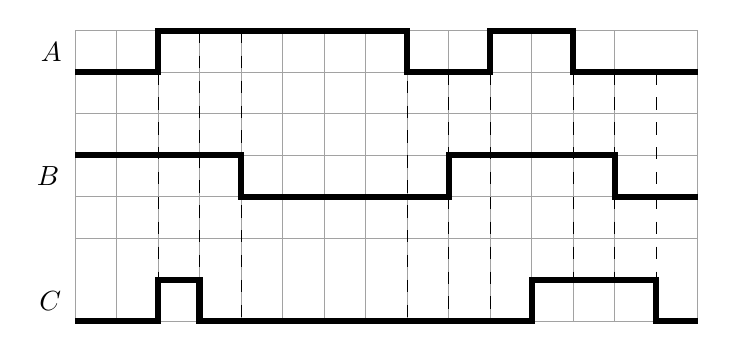
\begin{tikzpicture}[x=0.75pt,y=0.75pt,yscale=-1,xscale=1]
%uncomment if require: \path (0,300); %set diagram left start at 0, and has height of 300

%Shape: Grid [id:dp34531111101152123] 
\draw  [draw opacity=0] (100,40) -- (400,40) -- (400,180) -- (100,180) -- cycle ; \draw  [color={rgb, 255:red, 162; green, 162; blue, 162 }  ,draw opacity=1 ] (120,40) -- (120,180)(140,40) -- (140,180)(160,40) -- (160,180)(180,40) -- (180,180)(200,40) -- (200,180)(220,40) -- (220,180)(240,40) -- (240,180)(260,40) -- (260,180)(280,40) -- (280,180)(300,40) -- (300,180)(320,40) -- (320,180)(340,40) -- (340,180)(360,40) -- (360,180) ; \draw  [color={rgb, 255:red, 162; green, 162; blue, 162 }  ,draw opacity=1 ] (100,60) -- (400,60)(100,80) -- (400,80)(100,100) -- (400,100)(100,120) -- (400,120)(100,140) -- (400,140) ; \draw  [color={rgb, 255:red, 162; green, 162; blue, 162 }  ,draw opacity=1 ] (100,40) -- (400,40) -- (400,180) -- (100,180) -- cycle ;
%Straight Lines [id:da9908667716444586] 
\draw  [dash pattern={on 4.5pt off 4.5pt}]  (140,60) -- (140,160) ;


%Straight Lines [id:da9489034074703155] 
\draw  [dash pattern={on 4.5pt off 4.5pt}]  (160,40) -- (160,160) ;


%Straight Lines [id:da7444148673969375] 
\draw  [dash pattern={on 4.5pt off 4.5pt}]  (180,40) -- (180,180) ;


%Straight Lines [id:da33359589579811755] 
\draw  [dash pattern={on 4.5pt off 4.5pt}]  (260,40) -- (260,180) ;


%Straight Lines [id:da1689198722872045] 
\draw  [dash pattern={on 4.5pt off 4.5pt}]  (280,60) -- (280,180) ;


%Straight Lines [id:da2835936693187402] 
\draw  [dash pattern={on 4.5pt off 4.5pt}]  (300,60) -- (300,180) ;


%Straight Lines [id:da7069604701418795] 
\draw  [dash pattern={on 4.5pt off 4.5pt}]  (340,60) -- (340,160) ;


%Straight Lines [id:da35256438922338873] 
\draw  [dash pattern={on 4.5pt off 4.5pt}]  (360,60) -- (360,160) ;


%Straight Lines [id:da8396949759627998] 
\draw  [dash pattern={on 4.5pt off 4.5pt}]  (380,60) -- (380,160) ;


%Straight Lines [id:da8850959184881091] 
\draw [line width=2.25]    (100,60) -- (140,60) -- (140,40) -- (260,40) -- (260,60) -- (300,60) -- (300,40) -- (340,40) -- (340,60) -- (400,60) ;


%Straight Lines [id:da2574956876601695] 
\draw [line width=2.25]    (100,180) -- (140,180) -- (140,160) -- (160,160) -- (160,180) -- (320,180) -- (320,160) -- (380,160) -- (380,180) -- (400,180) ;


%Straight Lines [id:da8609754683162194] 
\draw [line width=2.25]    (100,100) -- (180,100) -- (180,120) -- (280,120) -- (280,100) -- (360,100) -- (360,120) -- (400,120) ;



% Text Node
\draw (88.5,50) node   {$A$};
% Text Node
\draw (87,110) node   {$B$};
% Text Node
\draw (88,170) node   {$C$};


\end{tikzpicture}
}

\hspace{0.5cm}

\begin{block}{}
\begin{minipage}{0.45\linewidth}
	\textbf{A função de transferência discreta de um sistema discreto é igual à sua resposta à entrada impulso}. Desta forma, para determinar $ G(z) $ devemos aplicar uma entrada impulsiva e obter a saída $ Y(z) $.
\end{minipage}
\hfill
\begin{minipage}{0.45\linewidth}
	\centering
	\scalebox{0.6}{
		\tikzmark{A}
	\deftkzbds

\begin{tikzpicture}[auto, node distance=1.5cm,>=Latex]
\node [input] (input2) {};
\node [block, right=of input] (computer) {$ G(z) $};
\node [output, right =of computer] (output2) {};
\node [above] at (input2) {$ U(z) $};
\node [above] at (output2) {$ Y(z) $};

\draw [->] (input2) -- (computer);
\draw [->] (computer) -- (output2);
\end{tikzpicture}}
\end{minipage}
\end{block}

\begin{tikzpicture}[remember picture, overlay]
\draw[<-] ($(A)+(2.15cm,0.61cm)$) -- +(0,2.5);
\end{tikzpicture}

\end{frame}


\begin{frame}{Segurador de ordem zero}
\begin{block}{}
O conversor D/A transforma o número binário em um nível de tensão que é mantido constante entre dois instantes sucessivos de amostragem pelo segurador de ordem zero \textbf{(ZOH)}.
\end{block}
\begin{minipage}{0.45\linewidth}
	\centering
	\scalebox{0.8}{
		\begin{tikzpicture}
	\draw[->] (-0.2,0) -- (5,0) node[right] {$kT$};
	\draw[->] (0,-0.2) -- (0,4.5) node[above] {$u(kT)$};
	
	\draw (0,0) ++(-0.16,-0.08) node[below] {$ 0 $};
	
	\foreach \x in {1,...,4}{
		\draw (\x,0) ++(0,-0.08) node[below] {$ \x T $} -- +(0,.16);
		\node[left] at (0,\x) {$ \x $};
		\draw (0,\x) ++(-0.08,0) -- +(.16,0);
	}
	
	\draw[] plot[only marks, mark=*, mark size=1.5pt] coordinates{(0,1) (1,2) (2,4) (3,3) (4,1)};
\end{tikzpicture}}\tikzmark{A}
\end{minipage}
\hfill
\begin{minipage}{0.45\linewidth}
	\centering
	\tikzmark{B}
	\scalebox{0.8}{
		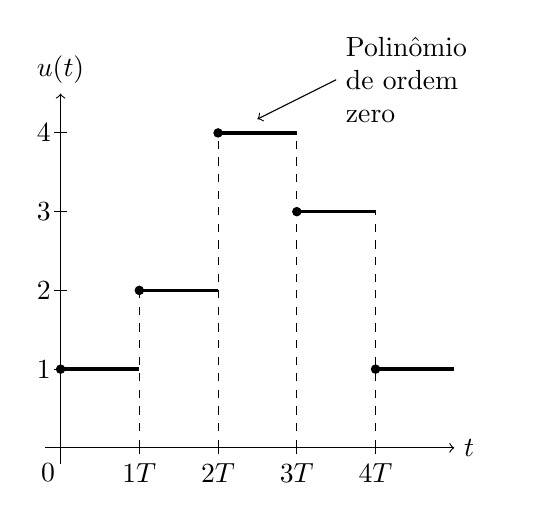
\begin{tikzpicture}
\draw[->] (-0.2,0) -- (5,0) node[right] {$t$};
\draw[->] (0,-0.2) -- (0,4.5) node[above] {$u(t)$};

\draw (0,0) ++(-0.16,-0.08) node[below] {$ 0 $};

\foreach \x in {1,...,4}{
	\draw (\x,0) ++(0,-0.08) node[below] {$ \x T $} -- +(0,.16);
	\node[left] at (0,\x) {$ \x $};
	\draw (0,\x) ++(-0.08,0) -- +(.16,0);
}

\draw[] plot[jump mark left, mark=*, mark size=1.5pt] coordinates{(0,1) (1,2) (2,4) (3,3) (4,1)};

\draw[line width=1.2pt] (0,1) -- (1,1) (1,2) -- (2,2) (2,4) -- (3,4) (3,3) -- (4,3) (4,1) -- (5,1);

\draw (4,1) -- +(0.8,0);

\draw[dashed] plot[ycomb, no marks] coordinates{(1,2) (2,4) (3,4) (4,3)};

\draw[<-] (2.5,4) ++(0,5pt) -- +(1,0.5) node[right,text width=2cm] {Polinômio de ordem zero};
\end{tikzpicture}}
\end{minipage}

\begin{tikzpicture}[overlay, remember picture]
\draw[->] (A) ++(-10pt,2cm) -- node[above] {D/A} +(1.3cm,0);
\end{tikzpicture}

\[ u(t)=u(kT)\, ,\quad kT\leqslant t<(k+1)T \]
\end{frame}


\begin{frame}{Segurador de ordem zero}
\begin{minipage}{0.45\linewidth}
	\centering
	\scalebox{0.8}{
		\begin{tikzpicture}
	\draw[->] (-0.2,0) -- (5,0) node[right] {$kT$};
	\draw[->] (0,-0.2) -- (0,4.5) node[above] {$u(kT)$};
	
	\draw (0,0) ++(-0.16,-0.08) node[below] {$ 0 $};

	\foreach \x in {1,...,4}{
		\draw (\x,0) ++(0,-0.08) node[below] {$ \x T $} -- +(0,.16);
	}
	
	\draw (0,2.25) ++(-0.08,0) node[left] {$ 1 $};
	
	\draw[] plot[only marks, mark=*, mark size=1.5pt] coordinates{(0,2.25)
		(1,0) (2,0) (3,0) (4,0)};
\end{tikzpicture}}\tikzmark{A}
\end{minipage}
\hfill
\begin{minipage}{0.45\linewidth}
	\centering
	\tikzmark{B}
	\scalebox{0.8}{
		\begin{tikzpicture}
	\draw[->] (-0.2,0) -- (5,0) node[right] {$t$};
	\draw[->] (0,-0.2) -- (0,4.5) node[above] {$u(t)$};
	
	\draw (0,0) ++(-0.16,-0.08) node[below] {$ 0 $};
	
	\foreach \x in {1,...,4}{
		\draw (\x,0) ++(0,-0.08) node[below] {$ \x T $} -- +(0,.16);
	}
	
	\draw (0,2.25) ++(-0.08,0) node[left] {$ 1 $};
	
	\draw[] plot[jump mark left, mark=*, mark size=1.5pt] coordinates{(0,2.25)
		 (1,0) (2,0) (3,0) (4,0)};
	
	\draw[line width=1.2pt] (0,2.25) -- (1,2.25) (1,0) -- (4,0);
	
	\draw (0,2.25) -- +(1,0);
	
	\draw[dashed] plot[ycomb, no marks] coordinates{(1,2.25)};
\end{tikzpicture}
		}
\end{minipage}

\begin{tikzpicture}[overlay, remember picture]
\draw[->] (A) ++(-10pt,2cm) -- node[above] {D/A} +(1.3cm,0);
\end{tikzpicture}

\begin{block}{Formulação matemática}
	A resposta do conversor D/A pode ser dada por $ u(t)=\underbrace{d(t)}_{\text{degrau}}{}-d(t-T) $
\end{block}
\end{frame}


\begin{frame}{Segurador de ordem zero}
\begin{block}{Formulação matemática}
Aplicando a transformada de Laplace em $ u(t) $ (entrada da planta $ G(s) $):
\begin{align*}
	\mathcal{L}\{u(t)\}&=\mathcal{L}\left\lbrace d(t)-d(t-T)\right\rbrace \\
				 U(s)&=\mathcal{L}\left\lbrace d(t)\right\rbrace -\mathcal{L}\left\lbrace d(t-T)\right\rbrace \\
				 U(s)&=\dfrac{1}{s}-\dfrac{1}{s}\text{e}^{-sT}\quad \text{, logo: }U(s)=\dfrac{1-\text{e}^{-sT}}{s}
\end{align*}

\[ Y(s)=G(s)U(s)\Rightarrow Y(s)=G(s)\cdot\dfrac{1-\text{e}^{-sT}}{s} \]

Logo, $ y(t)=\mathcal{L}^{-1}\left\lbrace \dfrac{1-\text{e}^{-sT}}{s}\cdot G(s)\right\rbrace  $
\end{block}
\end{frame}


\begin{frame}{Segurador de ordem zero}
	\begin{block}{Formulação matemática}
		Esta resposta passa pelo conversor A/D, gerando $  y(kT) $. Para isso, $t=kT$.
		
		\[ y(kT)=\eval{\mathcal{L}^{-1}\left\lbrace\dfrac{1-\text{e}^{-sT}}{s}\cdot G(s) \right\rbrace}_{t=kT}  \]
	\end{block}
\end{frame}


\begin{frame}{Segurador de ordem zero}
\begin{block}{Formulação matemática}
A transformada $\mathcal{Z}$ de $ y(kT) $ será:

\begin{align*}
	Y(z)&=\mathcal{Z}\left\lbrace y(kT) \right\rbrace=\mathcal{Z}\left\lbrace \eval{\mathcal{L}^{-1}\left\lbrace \left( 1-\text{e}^{-sT}\right) \cdot \dfrac{G(s)}{s} \right\rbrace}_{t=kT} \right\rbrace\\
	Y(z)&=\mathcal{Z}\left\lbrace\eval{\mathcal{L}^{-1}\left\lbrace \dfrac{G(s)}{s} \right\rbrace}_{t=kT}-\eval{\mathcal{L}^{-1}\left\lbrace\text{e}^{-sT}\cdot \dfrac{G(s)}{s} \right\rbrace}_{t=kT} \right\rbrace
\end{align*}
\end{block}
\end{frame}


\begin{frame}{Segurador de ordem zero}
\begin{block}{Formulação matemática}
Seja $ f(t)=\mathcal{L}^{-1}\left\lbrace \dfrac{G(s)}{s}\right\rbrace  $

\begin{align*}
Y(z)&=\mathcal{Z}\left\lbrace f(t)-f(t-T)\right\rbrace\Big|_{t=kT}=\mathcal{Z}\left\lbrace f(kT)-f(kT-T)\right\rbrace\\
Y(z)&=\mathcal{Z}\left\lbrace f(kT)\right\rbrace -\mathcal{Z}\left\lbrace f(kT-T)\right\rbrace\\
Y(z)&=\left( 1-z^{-1}\right) \mathcal{Z}\left\lbrace f(kT)\right\rbrace
\end{align*}

Porém $ f(kT)=\eval{\mathcal{L}^{-1}\left\lbrace \dfrac{G(s)}{s}\right\rbrace}_{t=kT} \quad $, logo:

\[ Y(z)=\left( 1-z^{-1}\right) \mathcal{Z}\left\lbrace \eval{\mathcal{L}^{-1}\left\lbrace \dfrac{G(s)}{s} \right\rbrace}_{t=kT}\right\rbrace \]
\end{block}
\end{frame}


\begin{frame}{Segurador de ordem zero}
\begin{block}{Formulação matemática}
	Como a resposta ao impulso $ Y(z) $ é igual a função de transferência do sistema $ G(z)$, temos que:
	
	\[ \boxed{G(z)=\left( 1-z^{-1}\right) \mathcal{Z}\left\lbrace \eval{\mathcal{L}^{-1}\left\lbrace \dfrac{G(s)}{s} \right\rbrace}_{t=kT}\right\rbrace} \]
\end{block}
\end{frame}


\begin{frame}{Segurador de ordem zero - Exemplo \#01}
\begin{block}{Problema}
Considere uma planta em tempo contínuo dada pela função de transferência
$$M(s) = \dfrac{s+3}{(s+1)(s+2)}$$
Determine o seu equivalente discreto utilizando o segurador de ordem zero e $T=\num{0,2}$ s.
\end{block}
\end{frame}

\begin{frame}{Segurador de ordem zero - Exemplo \#01}
\begin{block}{Resolução}
\begin{itemize}
    \item O primeiro passo é dividir $M(s)$ por $s$ e expandir em frações parciais:
\end{itemize}
$$\dfrac{M(s)}{s}=\dfrac{s+3}{s(s+1)(s+2)}=\dfrac{A}{s}+\dfrac{B}{s+1}+\dfrac{C}{s+2}$$
\begin{align*}
A&=\eval{\dfrac{s+3}{\cancel{s}(s+1)(s+2)}\cdot \cancel{s}}_{s=0}=\num{1,5} \\ B&=\eval{\dfrac{s+3}{s\cancel{(s+1)}(s+2)}\cdot\cancel{(s+1)}}_{s=-1}=-2 \\
C&=\eval{\dfrac{s+3}{s(s+1)\cancel{(s+2)}}\cdot\cancel{(s+2)}}_{s=-2}=\num{0,5}
\end{align*}
\end{block}
\end{frame}

\begin{frame}{Segurador de ordem zero - Exemplo \#01}
\begin{block}{Resolução}
\begin{itemize}
    \item A transformada inversa de Laplace é:
\end{itemize}
$$\eval{\mathcal{L}^{-1}\left\lbrace \dfrac{M(s)}{s} \right\rbrace}_{t=kT} = \num{1,5}-2\text{e}^{-kT}+\num{0,5}\text{e}^{-2kT}$$
\begin{itemize}
    \item A transformada $\mathcal{Z}$ (via tabela) é:
\end{itemize}
$$\mathcal{Z}\left\lbrace \eval{\mathcal{L}^{-1}\left\lbrace \dfrac{M(s)}{s} \right\rbrace}_{t=kT}\right\rbrace = \num{1,5}\dfrac{z}{z-1} -2\dfrac{z}{z-\text{e}^{-T}}+\num{0,5}\dfrac{z}{z-\text{e}^{-2T}}$$
\end{block}
\end{frame}

\begin{frame}{Segurador de ordem zero - Exemplo \#01}
\begin{block}{Resolução}
\begin{itemize}
    \item Deste modo,
\end{itemize}
\begin{align*}
    M(z)&=\left( 1-z^{-1}\right) \mathcal{Z}\left\lbrace \eval{\mathcal{L}^{-1}\left\lbrace \dfrac{M(s)}{s} \right\rbrace}_{t=kT}\right\rbrace \\
    &=\left(\dfrac{z-1}{z}\right) \left[ \num{1,5}\dfrac{z}{z-1} -2\dfrac{z}{z-\text{e}^{-T}}+\num{0,5}\dfrac{z}{z-\text{e}^{-2T}} \right] \\
    &=\num{1,5}-2\dfrac{(z-1)}{z-\num{0,8187}}+\num{0,5}\dfrac{(z-1)}{z-\num{0,6703}} \\
    &=\dfrac{\num{0,1977}z - \num{0,1081}}{z^2-\num{1,4890}z + \num{0,5488}}
\end{align*}
\end{block}
\end{frame}

\cprotect\frame{
\frametitle{\MATLAB}
\begin{block}{}
\begin{verbatim}
>>c2d(sys,T,'zoh') 
\end{verbatim}
converte um sistema dinâmico de tempo contínuo \textbf{sys} em tempo discreto com um tempo de amostragem $\bm{T}$ utilizando o método \textbf{zoh}. \\
\vspace{0.2cm}
\textbf{Exemplo}: discretização do exemplo \#01
\end{block}
\centerline{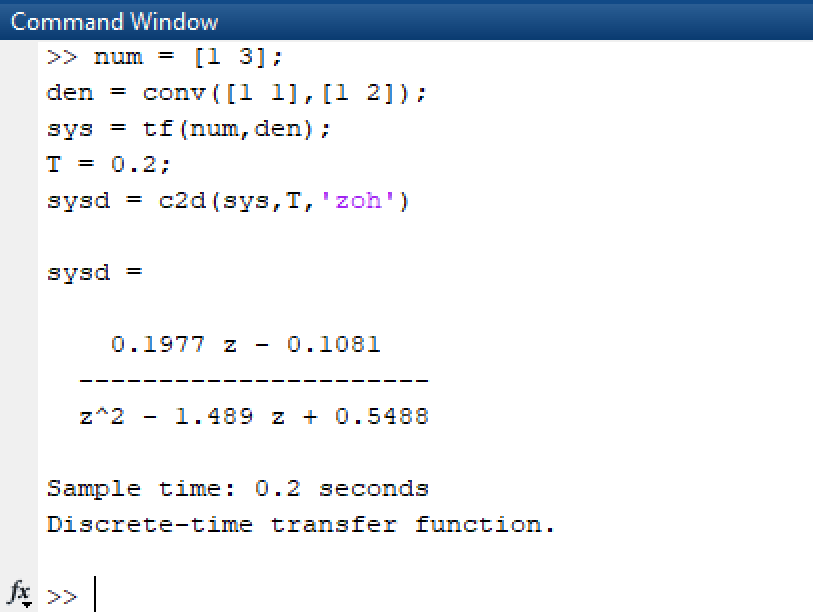
\includegraphics[width=0.55\linewidth]{Figuras/Ch06/fig1.PNG}}
}

\begin{frame}{Segurador de ordem zero - Exemplo \#02}
\begin{block}{Problema}
Considerando o sistema de controle digital abaixo e $ T=\SI{0.1}{\second} $, \textbf{determine se o sistema é estável}.

\vspace{0.5cm}

A planta é um motor DC cuja função de transferência é $G(s)=\dfrac{1}{s+1}$
\end{block}

\vspace{0.5cm}

\centering

\scalebox{0.8}{\deftkzbds
		
\begin{tikzpicture}[auto, node distance=2cm,>=Latex]
	% We start by placing the blocks
	\node [input] (input) {};
	\node [block, right=of input, xshift=0cm, align=center, text width=2cm] (computer) {$ h[n] $};
	\node [output, right =of computer] (output) {};
	\node [above, xshift=0.8cm] at (input) {$ x\left[n \right]  $};
	\node [above, xshift=-1cm] at (output) {$ y\left[n \right]  $};
	
	\draw [->] (input) -- (computer);
	\draw [->] (computer) -- (output);
\end{tikzpicture}}
\end{frame}

\begin{frame}{Segurador de ordem zero - Exemplo \#02}
\begin{block}{Resolução}
\begin{itemize}
    \item O primeiro passo é dividir $G(s)$ por $s$ e expandir em frações parciais:
\end{itemize}
$$\dfrac{G(s)}{s}=\dfrac{1}{s(s+1)}=\dfrac{A}{s}+\dfrac{B}{s+1}$$
\begin{align*}
A&=\eval{\dfrac{1}{\cancel{s}(s+1)}\cdot \cancel{s}}_{s=0}=1 \\ B&=\eval{\dfrac{1}{s\cancel{(s+1)}}\cdot\cancel{(s+1)}}_{s=-1}=-1 \\
\end{align*}
\end{block}
\end{frame}

\begin{frame}{Segurador de ordem zero - Exemplo \#02}
\begin{block}{Resolução}
\begin{itemize}
    \item A transformada inversa de Laplace é:
\end{itemize}
$$\eval{\mathcal{L}^{-1}\left\lbrace \dfrac{G(s)}{s} \right\rbrace}_{t=kT} = 1-\text{e}^{-kT}$$
\begin{itemize}
    \item A transformada $\mathcal{Z}$ (via tabela) é:
\end{itemize}
$$\mathcal{Z}\left\lbrace \eval{\mathcal{L}^{-1}\left\lbrace \dfrac{G(s)}{s} \right\rbrace}_{t=kT}\right\rbrace = \dfrac{z}{z-1} -\dfrac{z}{z-\text{e}^{-T}}$$
\end{block}
\end{frame}

\begin{frame}{Segurador de ordem zero - Exemplo \#02}
\begin{block}{Resolução}
\begin{itemize}
    \item Deste modo,
\end{itemize}
\begin{align*}
    G(z)&=\left( 1-z^{-1}\right) \mathcal{Z}\left\lbrace \eval{\mathcal{L}^{-1}\left\lbrace \dfrac{G(s)}{s} \right\rbrace}_{t=kT}\right\rbrace \\
    &=\left(\dfrac{z-1}{z}\right) \left[ \dfrac{z}{z-1} -\dfrac{z}{z-\text{e}^{-T}} \right] \\
    &=1-\dfrac{(z-1)}{z-\num{0,9048}} \\
    &=\dfrac{\num{0,0952}}{z-\num{0,9048}}
\end{align*}
\end{block}
\end{frame}

\begin{frame}{Segurador de ordem zero - Exemplo \#02}
\begin{block}{Resolução}
\begin{itemize}
    \item A função de transferência de malha fechada é dada por:
\end{itemize}
$$\dfrac{Y(z)}{R(z)}=\dfrac{\dfrac{z}{z-1}\cdot\dfrac{\num{0,0952}}{(z-\num{0,9048})}}{1+\dfrac{z}{z-1}\cdot\dfrac{\num{0,0952}}{(z-\num{0,9048})}}=\dfrac{\num{0,0952}z}{z^{2}-\num{1,8096}z+\num{0,9048}}$$
\begin{itemize}
    \item Para analisar a estabilidade do sistema (\textit{maiores informações no próximo capítulo}), podemos encontrar os polos da função de transferência de malha fechada, que são:
\end{itemize}
\begin{align*}
\text{Polos @ }z_{1,2}&=\dfrac{\num{1,8096}\pm\sqrt{\num{1,8096}^{2}-4\cdot1\cdot\num{0,9048}}}{2}\\
			   z_{1,2}&=\num{0,9048}\pm j\num{0,2935}\\
\left| z_{1,2} \right|&=\num{0,95}<1 \Rightarrow \text{\textbf{Estável}} 	
\end{align*}
\end{block}
\end{frame}

\begin{frame}{Desempenho de sistemas realimentados}
\begin{block}{Regime transiente e estado estacionário}
\begin{itemize}
    \item A resposta forçada de um  sistema dinâmico estável pode ser dividida em duas fases: o \textbf{regime transiente} e o \textbf{estado estacionário}.
    \item O \textbf{regime transiente} compreende o período de transição entre uma condição de operação estacionária e a seguinte, sendo que a mudança pode ter sido provocada por uma alteração na entrada do sistema ou pela ação de um distúrbio.
    \item O \textbf{estado estacionário} é a condição de operação permanente, da qual o sistema não sairá, a menos que alguma outra ação seja efetuada sobre ele. Por essa razão, o estado estacionário é também chamado de \textbf{regime permanente}. É importante notar que o estado estacionário não implica que a saída do sistema seja constante, mas significa que o padrão de comportamento não mais mudará, até que uma nova mudança seja necessária ou  provocada.
\end{itemize}
\end{block}
\end{frame}

\begin{frame}{Erro em regime permanente}
	\centering
	
	\scalebox{0.8}{\deftkzbds

\begin{tikzpicture}[auto, node distance=2cm,>=Latex]
	% We start by placing the blocks
	\node [input] (input) {};
	\node [block, right=of input, xshift=0cm, align=center, text width=2cm] (computer) {$ h[n] $};
	\node [output, right =of computer] (output) {};
	\node [above, xshift=0.8cm] at (input) {$ z^{n} $};
	\node [above, xshift=-1cm] at (output) {$ H(z)z^{n} $};
	
	\draw [->] (input) -- (computer);
	\draw [->] (computer) -- (output);
\end{tikzpicture}}
	
\begin{block}{Formulação matemática}
	\begin{align*}
		E(z)&=R(z)-F(z) \text{ e } F(z)=Y(z)H(z)\\
		E(z)&=R(z)-Y(z)H(z) \text{, mas }Y(z)=E(z)G(z)\\
		E(z)&=R(z)-E(z)G(z)H(z)\\
		E(z)+E(z)G(z)H(z)&=R(z)\\
		E(z)(1+G(z)H(z))&=R(z)\rightarrow \boxed{E(z)=\dfrac{R(z)}{1+G(z)H(z)}}
	\end{align*}
\end{block}
\end{frame}


\begin{frame}{Erro em regime permanente}
\begin{block}{Teorema do Valor Final (T.V.F.)}
\begin{itemize}
    \item Como o sistema é dinâmico, sabemos que não responderá instantaneamente a mudanças de referência.
    \item Mas o que ocorre em \textbf{estado estacionário}? À medida que o sistema se acomodar na nova condição de operação, será que o erro irá para zero? Essa situação pode ser analisada com o auxílio do teorema do valor final, que permite  escrever 
\end{itemize}
	\[ e(\infty)=\lim\limits_{k\to\infty}e(kT)=\lim\limits_{z\to1}(z-1)E(z) \]
\end{block}
\end{frame}


\begin{frame}{Erro em regime permanente}
\begin{block}{Entrada tipo degrau}
\begin{itemize}
    \item Considere uma entrada do tipo \textbf{degrau}:
\end{itemize}
$$R(z)=\dfrac{Az}{z-1}$$
	\begin{align*}
		e(\infty)&=\lim\limits_{z\to1}\cancel{(z-1)}\frac{Az}{\cancel{(z-1)}}\frac{1}{1+G(z)H(z)} \\
		&=\lim\limits_{z\to1}\frac{A}{1+G(z)H(z)}=\frac{A}{1+K_p}
	\end{align*}
	onde a \textbf{constante de erro de posição} é,
	\[ \boxed{K_p=\lim\limits_{z\to1} G(z)H(z)} \]
\end{block}
\end{frame}


\begin{frame}{Erro em regime permanente}
	\begin{block}{Entrada tipo degrau}
		\begin{itemize}
			\item Se $ G(z)H(z) $ não possui polo em $ z=1 $: $ K_p=\text{cte.} \Rightarrow e(\infty)=\text{cte.} $
			\item Se $ G(z)H(z) $ possui 1 polo em $ z=1 $: $ K_p\to \infty \Rightarrow e(\infty)\to 0 $
			\item Se $ G(z)H(z) $ possui 2 polos em $ z=1 $: $ K_p\to \infty \Rightarrow e(\infty)\to 0$
		\end{itemize}
	\end{block}
\end{frame}


\begin{frame}{Erro em regime permanente}
\begin{block}{Entrada tipo rampa}
\begin{itemize}
    \item Considere uma entrada do tipo \textbf{rampa}:
\end{itemize}
$$R(z)=\dfrac{ATz}{(z-1)^{2}}$$
	\begin{align*}
	e(\infty)&=\lim\limits_{z\to1}\cancel{(z-1)}\frac{ATz}{(z-1)^{\cancel{2}}}\frac{1}{1+G(z)H(z)}=\\
	&=\lim\limits_{z\to1}\frac{AT\cancelto{1}{z}}{\cancelto{0}{z-1}+G(z)H(z)(z-1)}=\lim\limits_{z\to1}\frac{AT}{(z-1)G(z)H(z)}=\dfrac{A}{K_v} 
	\end{align*}
	onde a \textbf{constante de erro de velocidade} é,
	\[ \boxed{K_v=\lim\limits_{z\to1}\frac{(z-1)G(z)H(z)}{T}} \]
\end{block}
\end{frame}


\begin{frame}{Erro em regime permanente}
	\begin{block}{Entrada tipo rampa}
		\begin{itemize}
			\item Se $ G(z)H(z) $ não possui polo em $ z=1 $: $ K_v=0 \Rightarrow e(\infty)=\infty $
			\item Se $ G(z)H(z) $ possui 1 polo em $ z=1 $: $ K_v=\text{cte.} \Rightarrow e(\infty) = \text{cte.} $
			\item Se $ G(z)H(z) $ possui 2 polos em $ z=1 $: $ K_v\to \infty \Rightarrow e(\infty)\to 0$
		\end{itemize}
	\end{block}
\end{frame}


\begin{frame}{Erro em regime permanente}
\begin{block}{Entrada tipo parábola}
\begin{itemize}
    \item Considere uma entrada do tipo \textbf{parábola}:
\end{itemize}
$$R(z)=\dfrac{AT^{2}z(z+1)}{2(z-1)^{3}}$$
	\begin{align*}
	e(\infty)&=\lim\limits_{z\to1}\cancel{(z-1)}\frac{AT^{2}z(z+1)}{2(z-1)^{\cancel{3} {\scriptscriptstyle 2}}}\frac{1}{1+G(z)H(z)}=\\
	&=\lim\limits_{z\to1}\dfrac{AT^{2}\cancelto{2}{z(z+1)}}{\cancelto{0}{2(z-1)^{2}}+G(z)H(z)2(z-1)^{2}}=\lim\limits_{z\to1}\dfrac{AT^{2}}{(z-1)^{2}G(z)H(z)}=
	\dfrac{A}{K_a}
	\end{align*}
	onde a \textbf{constante de erro de aceleração} é,
	\[ \boxed{K_a=\lim\limits_{z\to1}\frac{(z-1)^{2}G(z)H(z)}{T^{2}}} \] 
\end{block}
\end{frame}

\begin{frame}{Erro em regime permanente}
\begin{block}{Entrada tipo parábola}
	\begin{itemize}
		\item Se $ G(z)H(z) $ não possui nenhum polo em $ z=1 $: $ K_a= 0 \Rightarrow e(\infty)=\infty $
		\item Se $ G(z)H(z) $ possui 1 polo em $ z=1 $: $ K_a = 0 \Rightarrow e(\infty) = \infty $
		\item Se $ G(z)H(z) $ possui 2 polos em $ z=1 $: $ K_a = \text{cte.} \Rightarrow e(\infty) = \text{cte.}$
	\end{itemize}
\end{block}
\end{frame}

\begin{frame}{Erro em regime permanente}
\begin{block}{Conclusões parciais}
	\begin{itemize}
		\item Os erros serão tão menores quanto maiores forem as respectivas constantes (\textit{grandezas inversamente proporcionais}).
		\item Além disso, pelas definições dessas constantes, é possível ver que tais grandezas são definidas para \textbf{frequências que tendem a zero}.
		\item Em  outras palavras, a fim de reduzir o erro é necessário aumentar o ganho CC de ramo direto.
		\item Resumindo, \textbf{a redução de  erro em estado estacionário requer elevados ganhos em baixas frequências}.
		\item O aumento do ganho em baixas frequências \textbf{deteriora o desempenho transitório}, sendo que a malha pode até tornar-se \textbf{instável}.
	\end{itemize}
\end{block}
\end{frame}

\begin{frame}{Erro em regime permanente - Exemplo \#01}
\begin{block}{Problema}
Seja a função de transferência de malha aberta
$$G(z) = \dfrac{\num{0,15}(z+\num{0,5})}{z^2-z+\num{0,5}}$$
Para uma entrada degrau unitário, determine $K_p$, $e(\infty)$ e $y(\infty)$.
\end{block}
\end{frame}

\begin{frame}{Erro em regime permanente - Exemplo \#01}
\begin{block}{Resolução}
\begin{itemize}
    \item Para calcular $K_p$ usamos a fórmula:
\end{itemize}
$$K_p=\lim\limits_{z\to1} G(z)H(z) = \lim\limits_{z\to1}  \dfrac{\num{0,15}(z+\num{0,5})}{z^2-z+\num{0,5}} = \dfrac{\num{0,225}}{\num{0,5}} = \num{0,45}$$
\begin{itemize}
    \item O erro em regime permanente $e(\infty)$ para uma entrada degrau é:
\end{itemize}
$$e(\infty) = \dfrac{A}{1+K_p} = \dfrac{1}{1+\num{0,45}} \approx \num{0,69}$$
\begin{itemize}
    \item Sendo assim, como o erro é de aproximadamente $\num{0,69}$, temos que a saída em regime permanente $y(\infty)$ é calculada como:
\end{itemize}
$$y(\infty) = 1 - e(\infty) \approx \num{0,31}$$
\end{block}
\end{frame}

\begin{frame}{Erro em regime permanente - Exemplo \#01}
\begin{block}{Resolução}
\begin{itemize}
    \item Considere o acréscimo de um polo em $z=1$, com o objetivo de zerar o erro em regime permanente. Teríamos uma piora no regime transitório, como pode ser visto na simulação do sistema em malha fechada:
\end{itemize}
\end{block}
\centerline{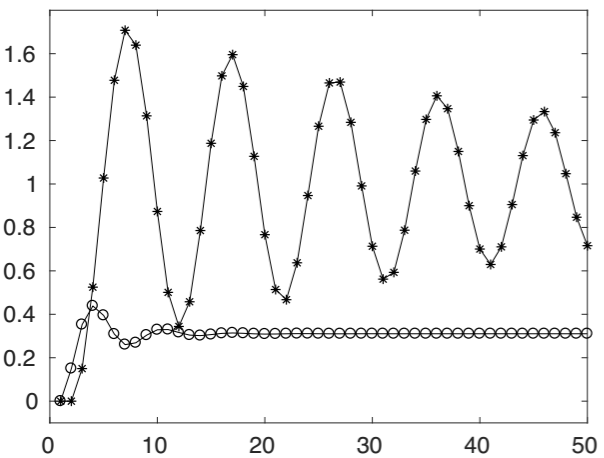
\includegraphics[width=0.6\linewidth]{Figuras/Ch06/fig2.PNG}}
\end{frame}

\begin{frame}{Erro em regime permanente - Exemplo \#01}
\begin{block}{Resolução}
\begin{itemize}
    \item Isto mostra o efeito da inclusão de um \textbf{integrador} (\textit{polo na origem}) na malha, ou seja, aumentar o tipo da função de transferência de malha, \textbf{melhora} a acurácia em \textbf{estado estacionário} em \textbf{detrimento} da \textbf{resposta transiente}.  
    \item Portanto, em projeto de sistemas de controle a inclusão de polos em $z = 1$ deve ser \textbf{compensado} de alguma forma de maneira a garantir uma \textbf{resposta transiente adequada}.
\end{itemize}
\end{block}
\end{frame}

\frame{
\frametitle{Exercícios}
\begin{block}{}
01. Qual é a transformada da planta $G(s)= a/(s + a)$ se o interpolador usado for o segurador de ordem zero com amostragem $T$?

\vspace{1cm}

02. Dado um sistema
$$G(s) = \dfrac{a}{s(s+a)},$$

determine as condições sob as quais o $K_v$ do sistema contínuo é aproximadamente igual ao $K_v$ do sistema precedido por um ZOH e representado por sua função de transferência discreta.
\end{block}
}

\frame{
\frametitle{Referências e exercícios complementares}
\begin{itemize}
\item AGUIRRE, Luis A. Controle de Sistemas Amostrados, 1 ed. [s.n.], 2019.
\end{itemize}
\centering{\alert{Página 125 - \textbf{Capítulo 4}}} \\
\centering{\alert{Página 234 - \textbf{Capítulo 6}}} \\
\vspace{0.4cm}
\begin{itemize}
\item FRANKLIN, Gene F.; POWELL, J. David; WOLKMAN, Michael L. Digital Control of Dynamic Systems, 3 ed. Addison-Wesley, 1998.
\end{itemize}
\centering{\alert{Página 270 - \textbf{Capítulo 7}}} \\
}